\section{Implications for physics-informed modelling}\label{sec:pinn}

\subsection{Which quantities the corpus actually contains}
Table~\ref{tab:physavail} audits the corpus against the quantities required by the standard
capacitance relations. The galvanostatic definition
\begin{equation}
C_g = \frac{I\,\Delta t}{m\,\Delta V}
\qquad\text{equivalently}\qquad
C_g = \frac{j\,\Delta t}{\Delta V},
\label{eq:gcd}
\end{equation}
and the cyclic-voltammetry relation
\begin{equation}
C_g = \frac{\int I(V)\,\mathrm{d}V}{m\,\nu\,\Delta V},
\label{eq:cv}
\end{equation}
both require a potential window $\Delta V$. That quantity, together with the discharge time
$\Delta t$, the absolute current $I$, the absolute electrode mass $m$, the electrode area and
the integrated CV current, is \textbf{entirely absent} from the corpus
(\texttt{electrode\_area\_cm2}, \texttt{voltage\_window\_V}, \texttt{current\_A}, \texttt{discharge\_time\_s}, all at
0\% coverage). The corpus does not even record whether a given row is a galvanostatic or a
voltammetric measurement.

\subsection{Assessment of three candidate model classes}
\paragraph{(A) Classical PDE/ODE-based PINN --- not justified.}
A physics-informed neural network in the usual sense~\cite{pinn2019} minimises the residual of
a differential
equation at collocation points, which requires a state variable defined over a space or time
coordinate together with initial and boundary conditions per observation. Every row in this
corpus is a single scalar summary of a completed experiment: there is no time axis, no
potential axis, no spatial coordinate and no trajectory. Without $\Delta V$ and $\Delta t$
even the \emph{algebraic} relation~\eqref{eq:gcd} cannot be evaluated for a single row,
let alone a differential form. Posing a PDE residual here would mean inventing physics rather
than enforcing it, and we therefore reject this option explicitly.

\paragraph{(B) Physics-guided neural network --- feasible.}
Positivity of capacitance, training-domain bounds and dimensionally meaningful inputs are all
available. Monotonicity constraints, however, should \emph{not} be imposed: the corpus shows
an interlayer-spacing trend opposite to the naive expectation (Sec.~\ref{sec:shap}), and
imposing a monotone prior from SHAP would encode a probable confound as physics.

\paragraph{(C) Hybrid physics-constrained multi-task regression --- recommended.}
Two exact algebraic closure identities relate the target to other measured quantities:
\begin{align}
C_A &= C_g\, m_A, \label{eq:areal}\\
C_V &= C_g\, \rho, \qquad \rho = m_A / t, \label{eq:vol}
\end{align}
where $m_A$ is areal mass loading, $t$ electrode thickness and $\rho$ the electrode density.
We verified both against the values reported in the source publications
(Table~\ref{tab:closure}). Equation~\eqref{eq:areal} reproduces the reported areal
capacitance with a median relative error of 0.38\% and holds within
5\% for 85\% of 39 testable rows;
Eq.~\eqref{eq:vol} has a median error of 0.87\% and holds within
5\% for 76\% of 34 rows.

This yields a structural insight that reframes two of the excluded columns. Areal and
volumetric capacitance cannot be \emph{predictors} --- they are algebraic transforms of the
target and were correctly removed as leakage --- but they can serve as \textbf{auxiliary
supervised outputs}, tied to the primary output by Eqs.~\eqref{eq:areal}
and~\eqref{eq:vol}. Two leakage columns thereby become additional training signal and a
genuine internal-consistency constraint, with no leakage introduced.

\subsection{Descriptor classification}
Table~\ref{tab:pinn} classifies every standardised descriptor.
\textbf{Category A} (physics-grade inputs): interlayer spacing (\AA), scan rate (mV\,s\textsuperscript{-1}), mass loading (mg\,cm\textsuperscript{-2}), electrode thickness ($\upmu$m) and H\textsubscript{2}SO\textsubscript{4} concentration (M). Mass loading and electrode
thickness qualify despite modest standalone SHAP importance because they appear directly in
the verified closure identities, entering the physics term rather than the data term.
\textbf{Category B} (machine-learning covariates only): layer morphology, composition family and gel electrolyte --- informative for
prediction, but categorical buckets with no counterpart in any governing relation, and
therefore excluded from every physics term.
\textbf{Category C} (excluded): current density (A\,g\textsuperscript{-1}), specific surface area (m\textsuperscript{2}\,g\textsuperscript{-1}), flake size ($\upmu$m), pore diameter (nm) and synthesis route, on grounds of
sparsity, absent variation, or non-convertible units, in addition to all target-derived and
metadata columns.

\subsection{Proposed formulation}
The recommended next-stage model (Fig.~\ref{fig:model}) predicts $\hat C_g$ through a
softplus output head, guaranteeing positivity by construction, with auxiliary heads for
$\hat C_A$ and $\hat C_V$. The objective is
\begin{equation}
\mathcal{L} = \lambda_{d}\mathcal{L}_{\mathrm{data}}
+ \lambda_{p}\mathcal{L}_{\mathrm{phys}}
+ \lambda_{b}\mathcal{L}_{\mathrm{bound}}
+ \lambda_{r}\lVert\theta\rVert^{2},
\label{eq:loss}
\end{equation}
with
\begin{align}
\mathcal{L}_{\mathrm{data}} &= \frac{1}{N}\sum_{i}
  \mathrm{Huber}\!\left(\hat C_{g,i}, C_{g,i}\right)
  + \sum_{o \in \{A,V\}} \frac{w_o}{|S_o|}\sum_{i \in S_o}
  \mathrm{Huber}\!\left(\hat C_{o,i}, C_{o,i}\right), \\
\mathcal{L}_{\mathrm{phys}} &= \frac{1}{|S_A|}\sum_{i \in S_A}
  \bigl(\hat C_{A,i} - \hat C_{g,i} m_{A,i}\bigr)^{2}
  + \frac{1}{|S_V|}\sum_{i \in S_V}
  \bigl(\hat C_{V,i} - \hat C_{g,i} m_{A,i}/t_i\bigr)^{2}, \\
\mathcal{L}_{\mathrm{bound}} &= \frac{1}{N}\sum_{i}
  \bigl[\max(0, -\hat C_{g,i})\bigr]^{2}
  + \frac{1}{N}\sum_{i} d_{\mathrm{hull}}(\mathbf{x}_i)^{2},
\end{align}
where $S_A$ and $S_V$ index the rows for which the required quantities are actually reported.
All physics residuals are masked in this way, so no value is imputed in order to satisfy a
constraint. A Huber data term is used rather than squared error because the corpus retains
genuine extreme values that a quadratic loss would allow to dominate. Evaluation remains
paper-grouped, and no synthetic rows are used.

\subsection{What would help most}
Table~\ref{tab:physavail} identifies the binding constraint, and the priority list in
\texttt{data\_gap\_priorities.csv} ranks the remedies. The two
highest-value additions are \emph{potential window} and \emph{discharge time}: at 0\%
coverage they are the only missing terms of Eq.~\eqref{eq:gcd}, and recovering them would
promote the physics term from a definitional unit closure applicable to a minority of rows to
the actual measurement equation applicable to every galvanostatic row. Recording the testing
mode would additionally separate galvanostatic from voltammetric measurements, which are
currently pooled.

\begin{figure*}[htbp]\centering
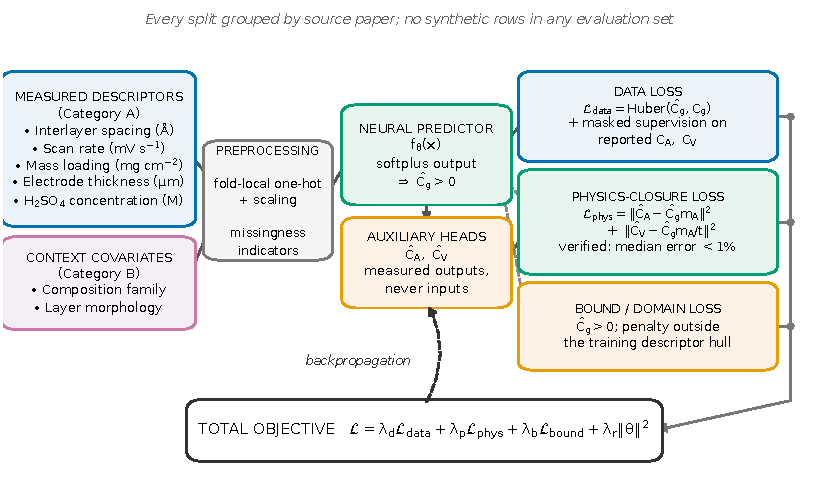
\includegraphics[width=\textwidth]{figures/fig09_proposed_physics_model.pdf}
\caption{Proposed hybrid physics-constrained multi-task architecture. Category~A descriptors
enter the predictor; Category~B covariates enter the data term only. Areal and volumetric
capacitance are auxiliary \emph{outputs}, never inputs, and are tied to the primary output by
the closure identities of Eqs.~\eqref{eq:areal}--\eqref{eq:vol}, which were verified against
the published values.}
\label{fig:model}\end{figure*}

\begin{table}[htbp]
\centering
\caption{Availability of the quantities required by the standard electrochemical capacitance relations, evaluated over the usable real observations.}
\label{tab:physavail}
\footnotesize
\begin{tabular}{llrrl}
\toprule
\textbf{Variable} & \textbf{Symbol} & \textbf{$n$} & \textbf{Coverage (\%)} & \textbf{Usable now} \\
\midrule
h2so4 M & $c0$ & 111 & 94 & yes \\
scan rate mV s & $nu$ & 88 & 75 & yes \\
interlayer A & $d$ & 88 & 75 & yes \\
volumetric capacitance F cm3 & $C\_V$ & 65 & 55 & yes \\
mass loading mg cm2 & $m\_A$ & 55 & 47 & partial - only 47\% of rows \\
electrode thickness um & $t$ & 54 & 46 & partial - only 46\% of rows \\
areal capacitance F cm2 & $C\_A$ & 46 & 39 & partial - only 39\% of rows \\
current density A g & $j$ & 35 & 30 & partial - only 30\% of rows \\
ssa m2 g & $S$ & 35 & 30 & partial - only 30\% of rows \\
electrode area cm2 & $A$ & 0 & 0 & no - variable is not present in the corpus at all \\
voltage window V & $dV$ & 0 & 0 & no - variable is not present in the corpus at all \\
current A & $I$ & 0 & 0 & no - variable is not present in the corpus at all \\
discharge time s & $dt$ & 0 & 0 & no - variable is not present in the corpus at all \\
electrode mass g & $m$ & 0 & 0 & no - variable is not present in the corpus at all \\
testing mode & -- & 0 & 0 & no - variable is not present in the corpus at all \\
cv current integral & $int(I dV)$ & 0 & 0 & no - variable is not present in the corpus at all \\
\bottomrule
\end{tabular}
\par\vspace{2pt}\begin{minipage}{\linewidth}\scriptsize Coverage is the fraction of usable rows for which the quantity can be parsed with an unambiguous unit. The four quantities required by $C_g = I\,\Delta t/(m\,\Delta V)$ that are entirely absent from the corpus are the reason a classical PDE-based PINN cannot presently be posed.\end{minipage}
\end{table}
\begin{table}[htbp]
\centering
\caption{Empirical verification of the algebraic capacitance closure identities against the values reported in the source publications. These identities are the physics that the corpus can actually enforce.}
\label{tab:closure}
\footnotesize
\begin{tabular}{lrrrrrr}
\toprule
\textbf{Closure identity} & \textbf{$n$ rows} & \textbf{Papers} & \textbf{Median err.\ (\%)} & \textbf{$<5\%$} & \textbf{$<20\%$} & \textbf{$>50\%$} \\
\midrule
$C_A = C_g \cdot m_A$ & 39 & 14 & 0.38 & 85 & 90 & 3 \\
$C_V = C_g \cdot m_A /t$ & 34 & 13 & 0.87 & 76 & 85 & 4 \\
\bottomrule
\end{tabular}
\par\vspace{2pt}\begin{minipage}{\linewidth}\scriptsize $m_A$ is areal mass loading and $t$ electrode thickness, so $m_A/t$ is the electrode density. Rows failing by more than 50\% are dominated by publications whose mass-loading convention differs from the one implied by their reported areal capacitance, which is itself evidence of cross-study protocol heterogeneity.\end{minipage}
\end{table}
\begin{table}[htbp]
\centering
\caption{Classification of every standardised descriptor for the next-stage physics-guided model. Category A: physically meaningful, well-covered and stable inputs. Category B: informative machine-learning covariates that are categorical proxies rather than physical parameters. Category C: excluded.}
\label{tab:pinn}
\footnotesize
\begin{tabular}{lrrlll}
\toprule
\textbf{Descriptor} & \textbf{SHAP rank} & \textbf{Miss.\ (\%)} & \textbf{Stability} & \textbf{Category} & \textbf{PINN input?} \\
\midrule
H\textsubscript{2}SO\textsubscript{4} conc.\ (M) & 2 & 6 & stable & A & yes \\
Scan rate (mV\,s$^{-1}$) & 3 & 25 & moderately stable & A & yes \\
Interlayer spacing (\AA) & 4 & 25 & moderately stable & A & yes \\
Electrode thickness ($\upmu$m) & 7 & 54 & stable & A & yes (closure) \\
Mass loading (mg\,cm$^{-2}$) & 10 & 53 & stable & A & yes (closure) \\
Composition family & 1 & 0 & stable & B & not directly \\
Layer morphology & 5 & 19 & stable & B & not directly \\
Gel electrolyte & 8 & 0 & unstable & B & not directly \\
Specific surface area (m$^2$\,g$^{-1}$) & 6 & 70 & moderately stable & C & no \\
Current density (A\,g$^{-1}$) & 9 & 70 & moderately stable & C & no \\
Pore diameter (nm) & 11 & 97 & moderately stable & C & no \\
Flake size ($\upmu$m) & 12 & 91 & moderately stable & C & no \\
Synthesis route & -- & 0 & not assessed & C & no \\
\bottomrule
\end{tabular}
\par\vspace{2pt}\begin{minipage}{\linewidth}\scriptsize Stability combines the cross-fold SHAP rank spread with the rank change observed between the real-only and Bayesian-augmented models. Full reasoning is in \texttt{results\_final/pinn/descriptor\_classification.csv}.\end{minipage}
\end{table}
